%% Hello emacs, this is -*- latex -*-
\typeout{ ====================================================================}
\typeout{ This is file conclusao.tex, created at 10-Sep-2006 }
\typeout{ Maintained by Andre Anjos <Andre.dos.Anjos@cern.ch> }
\typeout{ ====================================================================}

\chapter{Conclusões}
\label{chap:conclusions}

O Segundo Nível de Filtragem (LVL2) do Experimento ATLAS é um ambiente
extremamente complexo que deve operar, associado à eletrônica de leitura do
detetor, sobre elementos de deteção mais básicos no intuito de detetar canais
de decaimento do bóson de Higgs de maneira rápida e eficiente. Prevê-se que
apenas alguns bósons desta natureza sejam observáveis por hora, dada as
condições de operação do experimento. Esta Física, no entanto, se mostrará
escondida no meio de milhares de outros eventos ordinários. Para selecionar e
rotular os eventos \eng{online} neste árduo ambiente, o experimento contará
com um sistema de filtragem altamente especializado e otimizado, divido em 3
níveis conectados em cascata, com complexidade e tempo de processamento
crescentes. 

A taxa de aprovação de eventos do Primeiro Nível é sintonizada de acordo com a
capacidade de processamento nos demais níveis de filtragem do experimento, já
que realiza procedimentos de filtragem mais elementares não atingindo um nível
de eficiência tão especializado na Física de Interesse. Isto ocorre, dentre
outras razões pelo tempo limite de processamento para este nível, uma vez que
eventos gerados pelo LHC ocorrerão com um intervalo de apenas 25
nanossegundos. A taxa máxima de saída prevista para o LVL1 é de 100.000
eventos por segundo. Se cerca de 1000 nós de computação estiverem disponíveis
no LVL2, cada unidade de processamento deve se ocupar, nesta configuração, de
100 eventos por segundo para que se sustente a taxa de eventos do LVL1. Esta
taxa de execução representa uma média de tempo de processamento por evento de
apenas 10~milissegundos.

Dentre os canais de filtragem mais importantes para o experimento, estão
elétrons altamente energéticos (com mais que 10~GeV), que podem indicar muitos
tipos diferentes de decaimento para o bóson de Higgs. Cerca de 60 a 70\% das
assinaturas consideradas pelo LVL2 contém elétrons. Infelizmente a
contaminação de elétrons, por jatos com fortes componentes eletromagnéticas é
imensa na entrada do LVL2. Avalia-se que a cada 25.000 elétrons aprovados pelo
LVL1, apenas 1 seja um verdadeiro elétron! A relação sinal-ruído, nesta
condição é de $1/25000 = 4\times10^{-6}$.

A deteção de elétrons no LVL2 acontece, basicamente, em 2 etapas: uma análise
calorimétrica e uma análise de traços. Na análise calorimétrica, que encabeça
o processo de deteção, os dados presentes nos calorímetros são utilizados para
determinar o perfil de deposição energética da partícula analisada, de forma a
discriminá-la. Cada região analisada possui cerca de 1300 sensores (células)
que amostram a energia da partícula que passa pelo seu volume.

Para acessar os dados, os algoritmos devem se comunicar via rede com o sistema
de leitura do detetor, recortando a região necessária para sua
avaliação. Neste sistema distribuído, considerações importantes devem ser
feitas quando se avalia o tempo de processamento de um algoritmo. Sistemas que
necessitem de grandes quantidades de dados serão implicitamente mais lentos
que aqueles que conseguirem atingir uma decisão com menos informação e
portanto menos interessantes. Por outro lado, por causa das falhas inerentes a
um sistema com tamanha complexidade, deseja-se que os algoritmos atinjam
níveis de robutez capazes de suportar condições extremas (e.g. falha de
algumas células dos calorímetros). Ademais, uma vez que a Física de interesse
esteja embebida em um \textit{mar} de eventos ordinários, e que, acima de
tudo, seja desconhecida, almeja-se criar um sistema que consiga reconhecer
padrões em eventos que nunca dantes analisados.

A implementação do Sistema de Filtragem constitui-se, em si, outro desafio. O
transporte de dados entre as unidades de processamento deve ser assegurado por
uma implementação eficaz e robusta. Os algoritmos de filtragem propriamente
ditos, trabalham sob uma pilha de \eng{software} extremamente complexa que os
isola dos detalhes operacionais. A integração de um nova algoritmo de
filtragem com esta ``pilha'' também é, por si só, desafiadora.

Uma vez integrado e, em condições normais de operação os algoritmos de
filtragem baseados em calorimetria para o LVL2 devem lidar com outros
problemas: os dados disponíveis para análise são segmentados em camadas e,
dentro de uma mesma camada, há variação de granularidade dos sensores, que vão
se tornando mais largos à medida que se aproxima das bordas do detetor. Todas
as imperfeições do sistema de deteção devem ser contempladas, incluindo
regiões sem elementos de deteção destinadas à passagem de cabos para os
detetores internos. Com a aproximação do ``Dia 1'' de operação do experimento,
todas estas garantias devem ser feitas pelos desenvolvedores do sistema.

Uma vez que dados reais, coletados dos detetores mediantes colisões
protônicas, não estejam disponíveis atualmente, simula-se, com os mais
rigorosos detalhes, as condições físicas que serão encontradas ao se operar o
experimento. Simulações recentes incluem informações muito mais completas e
complexas sobre a geometria do detetor, parâmetros de calibração e, mesmo
sobre detalhes de ruído inerentes à eletrônica de leitura. A disponibilidade
de \textbf{toda} a infraestrutura do Sistema de Leitura, ligada à dados
simulados com tamanha precisão tornou possível a conclusão deste trabalho de
longa data.

\section{Contribuições ao Sistema de Filtragem do ATLAS}

Este trabalho foi desenvolvido no contexto da frutífera colaboração entre o
CERN e a UFRJ. Durante a estadia no CERN participamos do desenvolvimento de
boa parte dos componentes do Segundo Nível do Sistema de Filtragem do
ATLAS. Em especial a infra-estrutura de base da Unidade de Processamento
merece destaque. O sistema é executado em múltiplas tarefas (\eng{threads}) de
processamento contendo uma fila de entrada que é partilhada por Tarefas
Trabalhadoras que executam os algoritmos de filtragem. Para acessar os dados,
cada Tarefa Trabalhadora comunica-se com o sistema de leitura através de uma
interface que isola-o do acesso à rede, controlando a entrada e saída de
informações do processador. As Figuras~\ref{fig:l2puarch} e
\ref{fig:l2sc-interaction} resumem esta arquitetura.

Para que possam arbitrariamente executar tanto \eng{offline}, quanto
\eng{online}, simplificando comparações de desempenho e o desenvolvimento,
desenvolvemos uma interface de ``cola'' entre o universo \eng{online}, onde
eventos fluem pela rede do Sistema de Filtragem e são controlados de forma
estrita e o universo \eng{offline} onde os algoritmos são desenvolvidos e
testados. O \eng{Steering Controller} pode transparentemente acoplar
bibliotecas Athena dentro da Unidade de Processamento do LVL2 de forma a
executar algoritmos desenvolvidos nesta plataforma. 

Testes de eficiência foram executados para que se assegurasse um tempo morto
mínimo ao experimento. Os resultados destes testes encontram-se na
Tabela~\ref{tab:l2sc}, e nas Figuras~\ref{fig:tns-4fig}, \ref{fig:tns-5fig},
\ref{fig:tns-6fig}, \ref{fig:tns-scale-burn} e \ref{fig:tns-7fig}. Uma das
constatações mais importantes detetados neste período de trabalho, que
influencia até hoje o desenvolvimento de algoritmos é que seja mais custosa a
transferência e pré-processamento dos dados primários de deteção (exemplo:
leitura das células de uma RoI e sua calibração) que o tempo gasto somando
agrupamentos, anéis ou tomando decisões. Isto pode ser facilmente verificado na
Figura~\ref{fig:l2sc-mu}.

Dentre as outras contribuições da colaboração encontra-se, igualmente o
desenvolvido do aplicativo chamado Pseudo-ROS ou pROS, que armazena o
resultado do processamento de todas as Unidades de Processamento do LVL2 até
que o Filtro de Eventos possa lê-los e processá-los. Esta aplicação deve ser
bastante robusta pois constitui-se de um ponto de falha único (só existe um
pROS para todo o Sistema de Filtragem). Este aplicativo é, junto com a L2PU
atualmente utilizado no experimento tal como projetado.

Também desenvolveu-se uma biblioteca de leitura e escrita universal para
ATLAS, chamada \texttt{eformat}. Uma das restrições no desenvolvimento deste
componente do sistema de filtragem é sua natureza complexa, e a necessidade de
que opere de forma rápida. Atualmente esta biblioteca é utilizada em todo o
experimento, tendo sido tomada como implementação de referência.

Outras participações inclue passam por contribuições de maior ou menor escala
no Sistema de Relatório de Erros da Coleção de Dados do ATLAS, o Sistema de
Configuração dos Altos Níveis de Filtragem \cite{aa:rt-05, aa:jinst-06} do
Sistema de Filtragem, testes do sistema com centenas de máquinas
\cite{aa:chep-06-01} ou com feixe dedicado \cite{aa:tns-06}. Estes e outras
referências de trabalhos executados neste período podem ser vistas no
Apêndice~\ref{ap:published}.

\section{Discriminação multi-variável baseada em calorimetria}

A filtragem elétron/jato no LVL2 do ATLAS apresenta um conjunto de elementos
com complexidade interessante: os dados são provenientes de milhares de
sensores (células do calorímetro) onde existe uma propagação ou mistura não
linear (penetração e decaimento) do sinal observado (elétron) através do
detetor. Jatos (ruído) são normalmente confundidos com o sinal que se deseja
detetar em proporções exorbitantes. Detetores de elétrons para este nível de
filtragem devem ser construídos de forma a utilizar a formatação segmentada
dos sensores, serem rápidos e robutos.

Desta forma, o problema da deteção de elétrons no LVL2 pode ser observada como
um problema de otimização. Duas fases podem ser bastante bem definidas segundo
a literatura disponível e as características de projeto deste sistema:

\begin{enumerate}
\item Extração de características, onde deseja-se definir um esquema de
compactação da entrada em um conjunto de variáveis altamente discriminantes e
que representem o evento analisado;
\item Hipótese ou Deteção, onde utiliza-se as informações extraídas na etapa
anterior para se determinar a natureza do evento em estudo.
\end{enumerate}

Este tipo de análise foi empregado ao longo dos Capítulos~\ref{chap:baseline}
e \ref{chap:neural} de forma extensiva. Estas duas fases de processamento são
problemas atuais em Engenharia de Processamento de Sinais: a Extração de
Características é normalmente chamada Extração de Componentes, Compressão ou
Compactação enquanto que a fase de Hipótese é normalmente denominada Deteção
ou Filtragem. Atualmente, a compactação ou extração de características é feita
de forma empírica no experimento. Um especialista \cite{nevski-calor-1992} com
o conhecimento do sistema deteção determina um conjunto de figuras de mérito
que o habilitam e detetar as partículas de interesse, amparados em observações
da Física destes objetos.

Em situações deste tipo, é claro, a capacidade de deteção de tal sistema
estará limitada às observações que podemos fazer do mundo e codificar através
de cortes em planos uni ou bi-dimensionais. Este o limite de nossa capacidade
de análise visual. Técnicas de análise multi-variável, neste meio, são ainda
empregadas de forma muito incipiente, como foi possível observar ao longo da
revisão da literatura, no Capítulo~\ref{chap:neural}. A análise de Componentes
Principais, por exemplo, é citada normalmente como Análise pela Matriz
Hessiana, embora seja amplamente conhecida pelo outro nome. Métodos neurais de
processamento utilizam técnicas de treinamento baseadas na retro-propagação
erros em sua forma mais clássica, excetuando-se algumas raras excessões.

Existe, num geral, um certo ``receio'' na comunidade de Física de Altas
Energias no emprego de técnicas modernas de deteção. A fundamentação das
hipóteses deve ser bem feita e os resultados, sempre amparados em evidência
física, tentando-se estabelecer uma relação direta entre a compactação e a
filtragem e fenômenos observáveis. 

Com todos estes parâmetros em conta, desenvolveu-se o conjunto de técnicas de
deteção propostas neste trabalho. A utilização da análise multi-variável,
passando por simples detetores lineares e redes neurais artificiais é
empregada juntamente a diferentes métodos de compactação. No
Capítulo~\ref{chap:baseline}, avalia-se o método atual de compactação (T2Calo)
e deteção (EGammaHypo) empregado no CERN, caracterizando-os com relação a
massa de eventos simulados disponível para o trabalho. Como colocando
anteriormente em algumas instâncias, esta massa de dados é bastante completa
no tocante a muitas características do detetor tais como a segmentação,
geometria (variação de granularidade) e a presença de ruído. Esta informação
não estava presente em outros trabalhos. 

Levando-se em conta o empirismo no desenvolvimento deste sistema, ainda
percebe-se impressionante capacidade de deteção: este sistema consegue atingir
91,85\% contra apenas 10,19\% de falso alarme na deteção de jatos. Estes
patamares de operação são definidos através de um método de otimização por uma
\textbf{longa} busca incessante na determinação de 4 patamares de corte
aplicados sucessivamente em 4 variáveis que contêm a informação necessária à
discriminação. Este processo de otimização é caracterizado, genericamente, em
\cite{daqnote00-02}.

Uma análise mais detalhada do comportamento deste algoritmo revela alguns de
seus problemas. A Figura~\ref{fig:eghypo-eta-scan-test} mostra que o sistema
não consegue recuperar a informação perdida na região do \eng{crack} dos
calorímetros, apresentando baixo desempenho nesta área. A análise por energia
conduzida na Figura~\ref{fig:eghypo-emet-scan-test} mostra que a capacidade de
deteção do sistema funciona bem na presença de dados que possam ser utilizados
no passo de otimização, mas em regiões mais carentes, não consegue generalizar
apresentando ainda sim, boa qualidade de separação entre as duas classes de
partículas (RoI acima de 90~GeV de energia).

Uma vez que as fases de extração (compactação) e hipótese (deteção ou
filtragem) estejam definidas individualmente, é possível uma ação em
passos. Num primeiro passo define-se que a análise multi-variável seja uma
técnica que iguale ou melhore o desempenho do sistema de filtragem,
apresentando como bônus, métodos bem definidos (e rápidos) para seu ajuste. De
fato, esta característica é fundamental em ambientes como o ATLAS, onde as
variações de luminosidade poderão exigir rápidas mudanças nas parametrizações
dos detetores. Uma vez que se dispõe de apenas 4 variáveis para a deteção, o
sistema mais simples possível, descartada a separação por cortes, é um detetor
baseado em uma simples transformação linear que maximize a distância entre as
classes de partículas e minimize a distância entre os exemplos em cada
classe. Este discriminador é popularmente conhecido como \textit{Discriminante
de Fisher} \cite{fisher} e pode ser deduzido através de um processo iterativo
de treinamento como o LMS. Testes realizados com este sistema indicam, uma
capacidade discriminativa compatível ao EGammaHypo: 90,77\% na deteção de
elétrons contra 9,79\% de falso alarme. Este sistema pode ser ajustado (ou
treinado) em cerca de 20 passos de treinamento (cerca 1 minuto em um PC
moderno) para maximizar seu poder de discriminação. A análise por $\eta$ e por
$\phi$ revelam as mesmas mazelas do detetor baseado no EGammaHypo, i.e., pouco
poder de generalização, principalmente em regiões com poucas amostras, e pouca
robustez. Pequenos mal-ajustes no ponto de corte podem fazer degradar o
desempenho do sistema. Isto se deve ao fato de que as duas classes de
partículas não sejam linearmente separáveis levando-se em conta as 4 variáveis
disponíveis, como ilustra as Figuras~\ref{fig:lms-test-output} e
\ref{fig:eratio-vs-rcore}.

Redes neurais artificiais podem exibir recortes mais sofisticados em um espaço
multi-variável. Seria, sem perda de generalização, possível, desta forma,
substituir o detetor linear utilizado por um detetor neural executando a mesma
função. Escolhe-se o método conhecido como Retro-Propagação de Erros
Resiliente \cite{rprop} (detalhado no Apêndice~\ref{ap:rna}) para treinarmos
este novo sistema. Este método tem uma vantagem grande sobre a
retro-propagação tradicional pois praticamente não necessita de
parametrização. O único elemento variável é o número de neurônios escondidos
na rede neural. Determina-se que o número ótimo de neurônios escondido é 4
neste caso. O detetor é treinado (várias vezes) donde chega-se a conclusão que
tal sistema apresenta um conjunto de características muitas vezes superior aos
estudados anteriormente. A qualidade de classificação (neste trabalho
estabelecida pelo produto SP) atinge um pico próximo aos outros
classificadores, indicando 92,38\% de eficiência na deteção de elétrons contra
9,05\% de falso alarme na deteção de jatos. Porém, o que destaca este detetor
com relação aos outros não está no poder de discriminação no pico, mas na
robustez que proporciona ao aumentar a distância inter-classes muito mais que
nos casos anteriores. Isto pode ser bem observado na
Figura~\ref{fig:best-t2calo-mlp-output}.

Uma vez estabelecido que sistemas neurais podem realizar um nível de separação
mais eficaz e robusto para o ATLAS, é possível re-pensar o sistema de
compactação de características de forma a tentar extrair mais informações das
partículas que as 4 variáveis providas. Por inspeção do código de execução do
T2Calo foi possível identificar um conjunto de outras 10 variáveis que
poderiam contribuir na identificação das partículas. Na sua maioria estas
variáveis detalham as deposições energéticas nas diferentes camadas dos
calorímetros e, uma das variáveis, em particular a largura dos objetos
detetados na 2\eira camada e.m.. Aglutinando-se estas variáveis ao processo
discriminativo e retreinado-se um detetor neural para separar elétrons e jatos
obteve-se um resultado ainda melhor: 94,79\% contra uma taxa de falso-alarme
de apenas 7,93\%. As análises por energia e geometria indicam comportamentos
similares aos dos detetores anteriores, sem grandes novidades.

A grande quantidade de variáveis introduzidas de uma só vez torna-se
preocupante: muito possivelmente a correlação (mesmo correlações de alta
ordem) entre estas variáveis seja grande. Por exemplo, há uma correlação óbvia
entre a energia na 2\eira camada e.m. e a energia total na seção e.m., já que
esta é a mais profunda camada desta seção, acumulando a maior parte da
energia. Introduz-se, então, a técnica de análise de relevância, que tenta
identificar, dentre as entradas disponíveis ao processo discriminativo aquelas
que sejam mais relevantes ao sistema de discriminação. Isso é feito,
normalmente \cite{relevance}, observando-se a variação causada na saída do
detetor ao substituirmos a variável de entrada por sua média.

Embora bastante correlacionadas, a relação entre o mapeamento entrada/saída de
um detetor e seu poder discriminativo não é idêntica. Desta forma, propomos
uma variação do processo de extração de relevância que atende a esta
diferença, calculando o impacto na capacidade discriminativa do detetor quando
uma variável é substituída por sua média. Para um detetor baseado nas 14
variáveis produzidas pelo T2Calo, as diferenças encontram-se, principalmente,
nas variáveis mais relevantes e na ordem. Para testarmos qual dos métodos
traduz-se em melhores resultados de discriminação executa-se uma poda nas
variáveis de entrada do detetor e treinam-se novos detetores baseados no
sub-espaço determinado pela poda, nas duas configurações. Neste caso, os
resultados da poda baseada na relevância de discriminação mostra resultados
superiores. A Figura~\ref{fig:t2calo-all-relev-cut-compare} resume os
resultados obtidos. Como é possível notar, a poda resultante da relevância de
discriminação obtém resultados melhores na faixa de interesse (deteção de
elétrons acima de 80\%).

Uma vez definidos as capacidades do sistema de compactação proposto pelo
T2Calo e desenvolvido técnicas genéricas para lidar com a possível explosão de
variáveis (após o processo de compactação da entrada), propõe-se um segundo
compactador baseado na soma em anéis que preserva a estrutura segmentada da
informação dos calorímetros provendo ainda sim um alto grau de compactação
(cerca de 10 vezes). Este sistema é modelado observando-se a forma como
elétrons interagem com a matéria. Este compactador permite ainda rápida
extração das componentes e a fatores como dados faltantes e variações de
granularidade. Por utilizarmos um detetor neural, espera-se que este método
seja capaz de recuperar detalhes mesmo onde o compactador, no intuito de
simplificarmos sua implementação, teve que aglutinar ou suprimir
informação. Bibliotecas para a extração de anéis de referência e para o
treinamento neural foram desenvolvidas, estando descritas no
Apêndice~\ref{ap:framework}.

Cem variáveis estão disponíveis ao sistema de classificação depois da operação
deste extrator na região de interesse. Detetores neurais são e treinados e
otimizados para detetar elétrons e jatos observando este novo conjunto de
variáveis com resultados muito bons, indicando uma capacidade de detetar
elétrons de 96,21\% contra apenas 3,44\% de falso-alarme na deteção de
jatos. A robustez é igualmente boa, como pode ser visto na
Figura~\ref{fig:ringer-mlp-output}, atingindo níveis de separação inter-classe
não observados anteriormente. Ademais, nota-se que este novo sistema pode
recupeara muito bem a informação perdida na região do \eng{crack} dos
detetores, o que os outros sistemas, baseados na informação do T2Calo, não
conseguiram, como mostra a Figura~\ref{fig:ringer-eta-phi}. 

A análise de relevância (de discriminação) deste novo sistema exibe algo novo,
que ainda não tinha sido observado até então: existem componentes cuja a
relevância seja negativa, indicando que estariam possivelmente atrapalhando o
sistema de deteção. Remove-se este conjunto de variáveis (38 no total),
formando um novo detetor com apenas 62 variáveis. Treina-se algumas redes
neurais preservando a mesma configuração e observa-se que sistematicamente os
resultados são superiores ao sistema anterior, exibindo não só uma
convergência mais rápida assim como uma melhor qualidade de deteção.

Numa segunda interação observa-se valores de relevância negativa. Novos
detetores são treinados baseados em uma segunda poda seguindo-se os mesmos
princípios. Novamente detetores (agora ligeiramente) mais eficientes emergem
indicando que a poda nestas condições seja benéfica ao processo
discriminativo. Ao final, o melhor dos detetores consegue identificar
corretamente 96,89\% dos elétrons contra apenas 2,93\% de falso-alarme tendo
um pouco menos de metade do número total de anéis iniciais.

Finalmente discutimos o processo de normalização seqüencial que havia sido
aplicado aos dados, como descreve a Tabela~\ref{tab:seq}. Calorímetros medem a
nergia de partículas ainda que estejamos interessados em desenvolver um método
que seja independente da energia. Como é possível observar na
Figura~\ref{fig:transverse-energy} a diferença entre as diversas regiões de
interesse analisadas são grandes. Um fator de normalização, que dependa
diretamente da energia da partícula faz-se, portanto, essencial. Um segundo
problema um pouco menos evidente também deve ser tratado: há uma diferença de
energia nos dados simulados. Enquanto elétrons são provenientes de simulações
de bósons de Higgs de 130~GeV, encontram-se espalhados na faixa energética que
vai de, aproximadamente 15~GeV (corte do LVL1) até 130~GeV. Os jatos
disponíveis para estudo tinham a energia fixa em 25~GeV. Desta forma, utilizar
fatores não normalizados para o estudo com classificadores multi-variável
introduziria uma polarização indesejada.

A normalização seqüencial tenta, ao mesmo tempo que removendo as diferenças
energéticas entre as RoIs, amplificar a informação na periferia do ponto
central de impacto de forma a melhorar a relação sinal/ruído nesta
região. Isto é feito pois sabe-se que as diferenças nos padrões de deposição
entre elétrons e jatos encontram-se nesta região. Para que seja possível a
utilização de tal processo de normalização (ou de fato qualquer outro
dependente da energia), podas na entrada devem ser realizadas com
cuidado. Deseja-se podar das bordas para o centro, sempre que possível,
evitando que se perca a informação entre anéis, uma vez que a normalização
depende deste fator. Neste momento tenta-se retomar a informação original de
relevância na Figura~\ref{fig:ringer-sp-relevance} e propor um mecanismo de
compactação que eliminasse o máximo possível de componentes ``negativas'', mas
que ao mesmo tempo evistasse buracos entre os anéis. Desta forma seria
possível minimizar o carregamento \textbf{e} o tratamento dos dados de uma só
vez. Este detetor, depois de duas iterações converge para um sistema que se
utiliza de apenas 14 dos 100 anéis originais. A informação da seção hadrônica,
por exemplo, é compactada em uma só camada. A partir destes 14 anéis de
deposição energética foi possível reconstruir a eficiência do detetor com 100
anéis, diminuindo a estrutura e complexidade do operador neural e, por
conseqüência, seu tempo de treinamento. Para este detetor final possui uma
capacidade de identificação de elétrons de $97,24$\% contra um falso-alarme de
apenas $2,93$\%. Este foi, muito a frente, o melhor resultado obtido até o
momento. O sistema, no entanto, é apenas um pouco mais complexo do que aqueles
que foram propostos utilizando o mecanismo de compactação provido pelo T2Calo,
melhorando em até 3 vezes a rejeição de ruído ao mesmo tempo que aumentando 7
pontos percentuais a deteção de sinal. A Figura~\ref{fig:roc-all} mostra um
resumo dos métodos e avanços na separação obtidos com o emprego da análise
multi-variável no problema da discriminação elétron/jato, no ATLAS.

\begin{figure}
\begin{center}
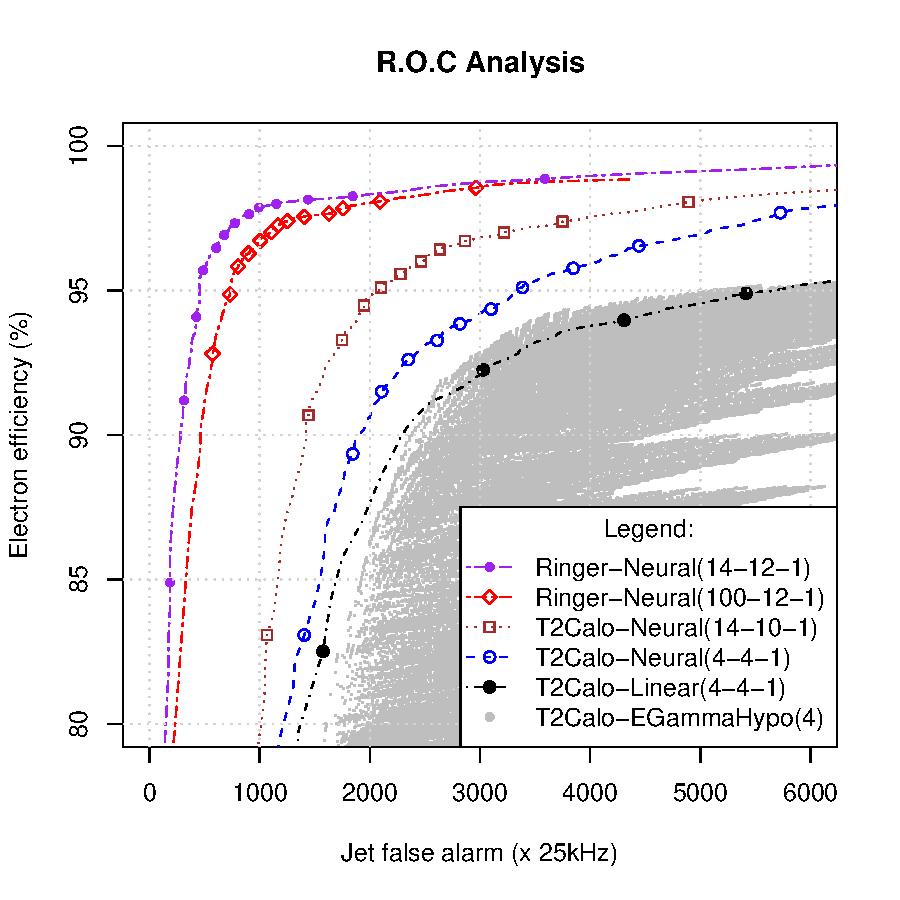
\includegraphics[scale=0.98]{roc-all}
\end{center}
\caption{Comparativo das curvas R.O.C. para os métodos de separação
elétron/jato baseados em análise multi-variável em comparação com o sistema
atualmente proposto no CERN.}
\label{fig:roc-all}
\end{figure}

Observando-se a análise de relevância deste último sistema baseado em 14
anéis, nota-se que as variáveis na periferia de cada região sejam as mais
importantes, como havia sido originalmente previsto. Como teste de robustez, o
mais relevante dos anéis é então artificialmente removido do conjunto de dados
de forma a se observar se um detetor baseado num espaço de entrada reduzido
conseguiria recuperar a informação perdida através dos outros anéis
sobreviventes. Os resultados são positivos: o novo detetor, formado dos 13
anéis menos relevantes obtém 97,59\% de eficiência na deteção de elétrons para
um falso-alarme na deteção de jatos de 3,22\% (SP=$1,83$), sendo apenas
marginalmente pior que aquele com 14 anéis. Este resultado indica que o
sistema possua algum nível de robustez.

\section{Implementação do detetor no ambiente de filtragem do ATLAS}

O último passo que demonstra a viabilidade de tal sistema é uma implementação
de referência dentro da pilha de \eng{software} do Sistema de Filtragem. Para
tal desenvolveu-se um conjunto de bibliotecas (veja o
Apêndice~\ref{ap:framework}) que implementam os procedimentos de anelamento e
deteção neural de forma independente. Este conjunto de bibliotecas pode ser
usado de forma desacoplada ao Sistema de Filtragem para o treinamento e
execução de detetores elétron/jato, formando um ambiente de desenvolvimento
rápido e eficiente. O tempo de execução em diferentes plataformas foi
aferido. Para a máquina mais rápida, o tempo necessário para gerar 100 anéis e
detetar elétrons por vias neurais é de cerca de 450 microssegundos. Utilizando
a última configuração, com apenas 14 anéis, o tempo de processamento cai para
meros 125 microssegundos, o que está bastante abaixo do que é requerido pelo
experimento, em quaisquer dos casos.

Uma vez que tenha sido construído tendo em vista a integração com o
experimento, estas bibliotecas também podem ser executadas dentro do ambiente
Athena e, por conseqÜência dentro do Sistema de Filtragem, utilizando-se de
toda a infraestrutura de acesso e tratamento aos dados disponível. Dois
algoritmos distintos são desenvolvidos baseado-se no conjunto de bibliotecas
do \eng{NeuralRinger}: um algoritmo de Extração de Características
(\texttt{HLTFEx}), que gera os anéis e um segundo (\texttt{HLTHypo}) que
implementa a deteção neural. Ainda que embebidos nesta nova infraestrutura de
processamento os sistemas continuam completamente flexíveis e configuráveis,
podendo eventualmente atender a outros problemas de filtragem no
experimento. O código faz parte, atualmente, do repositório central de
\eng{software} para o experimento.

Um conjunto de validações das entradas e saídas destes blocos operacionais é
conduzida, o que indica que o sistema esteja operando exatamente como em sua
forma desacoplada (Figuras~\ref{fig:athena-vs-nr} e
\ref{fig:athena-vs-nr-full}). A Figura~\ref{fig:timings-athena} resume os
resultados de tempo obtidos nesta fase. Para a extração de anéis e deteção
neural integrada, o tempo de processamento excluindo o acesso e calibração dos
dados é de cerca de 800 microssegundos, 60\% maior que na implementação
desacoplada. Esta penalização no tempo de processamento ocorre em detrimento
da pesada estrutura em \eng{software} que garante uma execução robusta no
Sistema de Filtragem - é o ``preço'' a ser pago. O tempo de accesso aos dados
não pode ser considerado neste exercício uma vez que, neste caso, os dados
estejam sendo lidos de um disco local ao invés de diretamente do Sistema de
Leitura do detetor.

O passo seguinte é a execução do sistema distribuído de filtragem, que emule
de forma ainda mais precisa a execução dentro do Sistema de
Filtragem. Desenvolve-se uma bancada de testes como mostra a
Figura~\ref{fig:online-schema}. Disparam-se 8 unidades de processamento do
LVL2 paralelamente executando os procedimentos de anelamento e deteção neural,
usando-se a infraestrutura de histogramas \eng{online} para monitorar o tempo
de execução do algoritmo de anelamento. De fato, sabe-se que não haverá
mudanças no tempo de processamento da parte de extração neural uma vez que não
acessa dados remotos à L2PU, sendo os tempos encontrados anteriormente ainda
válidos para esta análise. A Figura~\ref{fig:ringer-screenshot} mostra,
finalmente, uma captura de tela onde o sistema de anelamento e extração neural
encontram-se em execução dentro da bancada de testes. Como é possível notar a
partir do histograma produzido \eng{online}, o tempo de processamento do
algoritmo, incluindo acesso à dados, é de 3,8 milissegundos, que é compatível
com o tempo de execução atual do T2Calo, de 3,64 milissegundos, para obter uma
eficiência de classificação melhor, com 3 vezes maior nível de rejeição.

\section{Conclusões finais}

Com base em simulações mais realísticas do sistema de deteção e da Física que
ocorrerá dentro no experimento ATLAS, que procura a existência do bóson de
Higgs, foi possível desenvolver esquemas de deteção elétron/jato muito mais
eficientes e robustos que o atualmente proposto no CERN. Este sistema é
flexível e compactável (de 1300 células para 14 anéis apenas) através de um
processo simples, baseado no poder de discriminação do próprio detetor, que
maximiza o poder de discriminação e miniza as perdas de compactação. Os
detetores são projetados utilizando-se técnicas modernas de análise
estatística, introduzindo um novo conjunto de ferramentas dentro do campo de
Física de Altas Energias.

A informação para a discriminação encontra-se geometricamente segmentada,
possuindo, em diferentes casos, variações de granularidade importantes que
foram consideradas pelos métodos de deteção. As simulações disponíveis
continham, dentre outras, a informação de ruído tal qual estará presente
durante o experimento. O sistema desenvolvido utiliza técnicas modernas de
deteção multi-variável, podendo ser implementado e ajustado para as diversas
fases de operação do experimento, sem necessitar a intervenção de um
especialista. Este sistema foi implementado dentro da pilha de \eng{software}
do ATLAS, demonstrando que poderia ser executado em limites de tempo cabíveis
para operação no Segundo Nível de Filtragem, segundo vários critérios.

\section{Linhas de pesquisa}

A Análise de Componentes Principais, aplicada ao problema da separação
elétron/jato através dos dados de uma RoI ou através da informação de anéis,
foi abordada em uma tese de doutorado \cite{herman}, com bons
resultados. Nesta análise, desejou-se obter um sistema de compactação da
informação contida em RoIs através da aplicação direta da análise de
componentes principais sob as células na região de interesse ou sob a soma em
anéis desenvolvidas neste trabalho. Esta abordagem tenta, através da
transformação linear que descorrelaciona as diversas variáveis de entrada de
um detetor, encontrar traços das componentes físicas originárias de uma
partícula, que a caracterizem eficientemente.

A Análise de Componentes Independentes representa uma extensão da Análise de
Componentes Principais \cite{oja-ica}. Desta vez, no lugar de se procurar uma
transformação linear que descorrelacione o espaço transformado, deseja-se
computar a transformação linear na qual as variáveis do espaço transformado
tornem-se independentes. Esta é uma premissa muito mais forte que a simples
descorrelação, pois implica que a estatística que relacione quaisquer duas
variáveis do conjunto transformado será nula, para todos os graus
estatísticos.

Uma das pré-condições para que seja Análise de Componentes Independentes (ACI)
é de que o ruído introduzido pelo sistema no sinal de análise seja branco e
gaussiano. Esta é, no entanto, uma hipótese bastante razoável em experimentos
de física de altas energias \cite{knoll, leo}. A ACI pode ser conduzida
utilizando-se diversos métodos, que deverão ser avaliados com relação a sua
velocidade e qualidade.

O conjunto de componentes extraídas não poderá ser organizado, \textit{a
priori}, como acontece no caso da Análise de Componentes Principais, já que
não há uma correlação evidente entre os coeficientes da transformação e sua
importância. Neste caso, outros métodos, como o método da relevância de
discriminação introduzido neste trabalho, poderão ser explorados para que se
atinja a compactação dos dados de entrada.

Espera-se que a ACI possa relevar informações no padrão de interação das
partículas com os calorímetros do ATLAS, que estão mascarados nas varíaveis de
entrada, aumentando assim a qualidade da discriminação conduzida no LVL2.

Métodos de treinamento mais sofisticados podem ser também introduzidos no
sistema atual de deteção neural, aumentando a qualidade do treinamento, tempo
de convergência e a robustez do sistema de discriminação final. Em especial,
técnicas mais modernas como redes neurais qüânticas \cite{qnns} ou menos
exploradas neste contexto, como máquinas de vetor de suporte \cite{haykin}
podem ser pensadas como alternativas interessantes.

A compactação baseada na soma em anéis de deposição energética pode ser
explorada de forma a ser maximizada. Novas combinações devem ser exploradas
tendo em vista a quantidade de dados que devam ser lidas do sistema de
leitura do detetor e o fator de compactação propriamente dito. Especificamente,
a técnica de normalização dos dados poderia ser ajustada tendo em vista os
resultados da análise de relevância.

Finalmente, a deteção baseada em anéis pode também ser utilizada para análise
e reconstrução \eng{offline}. O sistema de deteção desenvolvido neste trabalho
deve ser re-adaptado para trabalhar neste ambiente e comparativos diretos com
as técnicas atuais de reconstrução podem ser utilizados. Métodos
multi-variável são bastante utilizados atualmente nesta sub-área da Física de
Altas Energias.

\typeout{ *************** End of file conclusao.tex *************** }
